\documentclass[twocolumn]{report}
% \documentclass{report}

\title{Building and Validating A Gaze-Aware AI System for Automatic Paragraph-Level Bookmarking}
\author{Henry Ash Williams}
\date{\today}

\usepackage[backend=bibtex]{biblatex}
\usepackage[compact]{titlesec}
\usepackage{kpfonts}
\usepackage[margin=2cm]{geometry}
\usepackage{hyperref}
\usepackage{siunitx}
\usepackage{graphicx}

\addbibresource{references.bib}


\begin{document}
\maketitle
\tableofcontents

\chapter{Introduction}
% Objectives of the project 
% Intended users 
% Achievable (experience/time available)? 
% Introduce Problem Area 
% Overview of the rest of the report 

% Suggestion: write intro 3x, reader with no knowledge, reader of peers, expert in the area
% then make it read like one introduction 
% 1-2 pages 

\section{Aims}


When using a web browser, users often have to switch back and forth between tabs, sometimes to cross reference facts with other sources, other times to control music playing in the background. However, having someones focus switch between multiple web pages can easily lead to users forgetting their place in an article, and then having to waste time finding it again. My project seeks to solve this goal by developing a web browser extension which will enhance the reading experience by automatically detecting and highlighting the last paragraph read when users switch between browser tabs or otherwise has their focus taken away from the page. In order to achieve this goal, I will make use of a technique called Gaze Mapping. This technique typically utilizes a mix of both specialized hardware, and machine learning models to predict where a user is looking on a screen. While these solutions can achieve a high level of accuracy, $\ang{0.3}$ under ideal conditions \cite{tobiiprofusion}, they require users to buy specialized, and often expensive equipment. 

In order to make this technology more accessible, I aim on creating a more cost effective solution. My approach will make use of the existing cameras found in most modern devices, such as the web cam found in laptops, and front facing cameras found in smartphones. Thus enabling us to extend the benefits of this technology to a broader audience. 

\section{Motivation}

This project is motivated by the fact that there's no good way to automatically keep track of where you are in a large peice of text on digital devices, such as laptops and smartphones. 

My project seeks to solve this problem by visually showing users their place in text, utilizing AI and machine learning. 

The target user for this project is an individual who frequently read on their computers and face the challenge of losing their place in the text when switching tabs which can disrupt their workflow. 

\section{Specific Objectives}\label{sec:specific-objectives}

There are two specific tasks I want to accomplish as part of this project. Firstly, the development and evaluation of a machine learning model which predicts the location of a users gaze on a screen using images taken from their front facing camera. The second objective of this project is the development and validation of software which takes pictures from the users webcam whenever the current browser tab is taken out of focus and securely transmits the image to another application hosting the aforementioned machine learning model, and uses the models prediction in order to highlight the paragraph the user was reading last. 

The machine learning model should be able to make predictions within an approximate $2.5\text{cm}$ radius of the true gaze location, in order to accurately distinguish between paragraphs on the screen. 
\section{Stretch Objectives}

Stretch objectives are tasks that I consider to be optional. If I have achieved my main goals, as outlined in Section \ref{sec:specific-objectives}, and still have time before the final due date of the project, I will attempt to implement them. 

My stretch objectives include a more accurate machine learning model, with an average accuracy of approximately $1\text{cm}$ of the true gaze location. This will enable more accurate detection of paragraphs and could even be used to detect the readers place in the text on a per-line or even per word basis. 

As it currently stands, the locations of the paragraphs will be detected using the information provided from the document object model (DOM) of the webpage. However, I want this extension to work on documents which aren't written in HTML, such as PDFs. This would require a computer vision system to detect where paragraphs are in an image. This is a stretch objective as it requires implementing and testing another complex feature for the project.

\chapter{Professional and Ethical Considerations}

\noindent
The BCS code of conduct \cite{bcs2022coc} outlines a set of guidelines which IT professionals are expected to follow. These guidelines seek to improve the public image of ethical practices within the computing field. They include considerations relating to the interest of the public, professional competence and integrity, duty to the relevant authorities and the profession. This section will explore how I will ensure my project adheres to these guidelines. 

\section{Public Interest}   

In order to adhere to the requirements set out by BCS, my project must ensure that the health, privacy, security and well being of its users are respected. 

To ensure the privacy of users is respected, the software will not share any information with third parties, and will be fully encrypted while in transit between the web browser and the machine learning model. 

Furthermore, the images captured to facilitate gaze mapping will not be stored, and instead will immediately be discarded once they have been used by the machine learning model to predict their gaze location.

Users will be in complete control of the capture of these images and will be informed as to how the images will be used. However, if the user does not grant the application permission to use their devices camera, the extension will not function. 

In order to ensure the machine learning model behaves as expected for all users, the model will be trained on a diverse set of participants. The datasets I plan on using however include over 1500 unique participants, made up of people with diverse backgrounds. This should ensure the model learns how to function correctly for all users. 

The software will be freely available for all of the most commonly used browsers. This includes Google Chrome, Firefox, Microsoft Edge, and Opera. 

\section{Professional Competence \& Integrity}   

Section two of the BCS code of conduct outlines requirements relating to the professional competence and integrity of the person developing the software. The first three points within this section state that the project should be within your level of expertise, that you should not claim any level of competence that you do not posses, and that you should develop your skills and competence as part of the project. I have discussed my project with my supervisor, and we believe that this project is within my professional competence.

I have also researched the relevant legislation regarding user data and machine learning models, and will not violate any such legislation as part of this project. 

The code of conduct also states that alternative viewpoints, and honest criticism of work is respected and valued. I plan on regularly meeting with my supervisor in order to gain insight on my project and gather feedback as to how it could be better. 

I also understand that I must avoid injuring others, their property, reputation or employment by malicious or negligenct action or inaction. This includes respecting the rights of the authors of the datasets which I plan on using, and their participants. Every action I can possible make to ensure their rights are respected will be taken. 

Finally, I will not take or make bribes behave in unethical practices, and discourage other professionals from similar actions.  

\section{Duty to Relevant Authority}   

The project will be developed with the utmost care and respect for the academic policies of the University of Sussex. This includes avoiding potential conflicts of interest, and accepting responsibility for any that may arise during development. No confidential information will be disclosed without explicit permission of the University. Furthermore, no information will be misrepresented or withheld. 

\section{Duty to the Profession}   

As part of my duty to the profession, I commit to uphold the reputation of the profession by accepting personal responsibility and will ensure that no actions will harm its standing. This project will be dedicated to taking positive steps to enhance the professional standards of the profession and actively contributing to upholding the reputation of BCS. I will conduct myself with integrity and respect in all professional relationships with BCS members and others. Furthermore, I will be committed to fostering a supportive environment by encouraging and assisting others to uphold the same goals. 

\section{Ethical Application}

As part of this project, I have submitted an ethics application to ensure all the work I plan on doing is done in a manner where the rights of the participants are respected. The application assigned my project a low risk level, however, as of \today, I am yet to receive approval. 

\chapter{Methodology}

\section{Background Reading}

\noindent
In literature, terminology for eye tracking is used very inconsistently. For example, the phrase ``Gaze Estimation'' can be used to describe the 3 dimentional directional vector showing a users gaze direction in the world. In this paper, I use the phrase ``Gaze Mapping'' to describe the process of taking an image of the user and predicting a set of 2 dimentional coordinates which represent an area on the screen where the user is currently focussed on. The phrase ``Eye tracking'' may also be used to describe this process. 

I could not find any applications which deliver an automated paragraph level bookmarking system using eye tracking to suppliment this work, so my background reading mostly focussed on existing machine learning models designed for gaze mapping. However, I was able to find a study \cite{barzvi2020eyetrackingdigialreading} using eye tracking to compare how poor and typical readers interact with text. 


\subsection{iTracker}\label{sec:itracker}

As part of my background reading, I have looked at machine learning models performing gaze mapping in order to develop my knowledge of how existing approaches work. This includes the \verb|iTracker| model \cite{krafka2016eye} which helped me develop my understanding of how datasets are processed, and the structure of machine learning models built for these tasks. This model uses a Convolutional Neural Network which can achieve a prediction error of $1.71\text{cm}$ on mobile devices, and $2.53\text{cm}$ on tablet devices without the need for calibration. When a calibration step was included, the error can be reduced to $1.34\text{cm}$ and $2.12\text{cm}$ respectively. 

The model itself is made up of three convolutional neural networks, see Figure \ref{fig:itracker-model} , two with shared weights trainied on cropped images from the left and right eyes, one for the face. The model also takes in a binary mask of where the face is located in the image. These are then used to predict where on the screen the user is looking. As mentioned earlier, this model can achieve a high degree of accuracy. Furthermore, it was trained on a large dataset of over 1450 participants, meaning it is more robust to variations in lighting conditions, skin tone, and head position. 

\begin{figure}[h]
    \begin{center}
        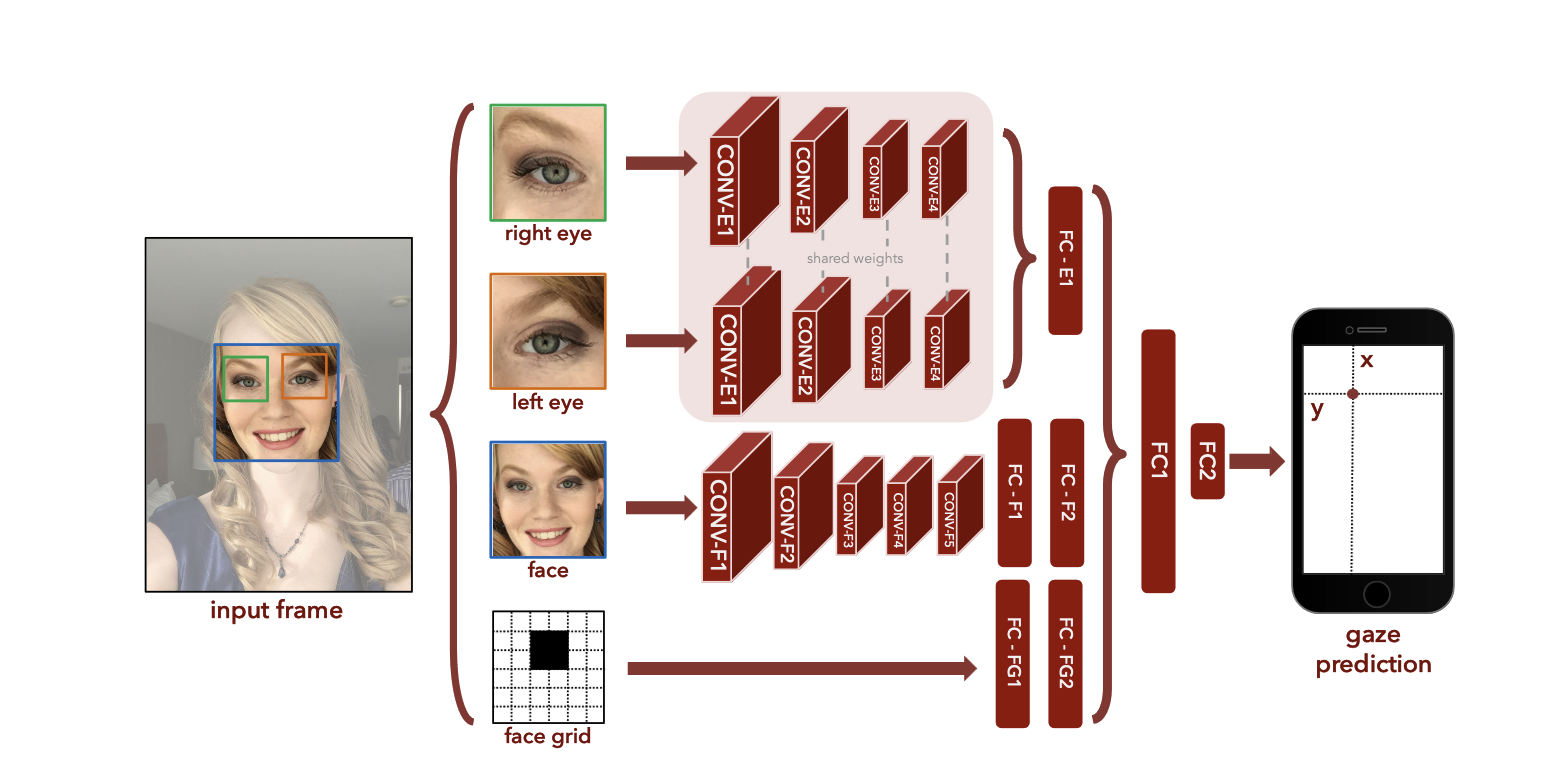
\includegraphics[scale=0.3]{../assets/iTracker-network.png}
    \end{center}
    \caption{The structure of the iTracker model, taken from ``Eye Tracking for Everyone'', 2016 \cite{krafka2016eye}}
    \label{fig:itracker-model}
\end{figure}

\subsection{Recurrent CNN for Gaze Estimation}

I also looked at some papers perfoming a different, yet related task. Namely Gaze Estimation \cite{palmero2018recurrent}, which estimates a vector representing where the user is looking in 3d space. However, as this does not provide information about where they are looking on the screen without estimating both the users and the devices position in 3d space, it's not very helpful in my use case. 

\subsection{Eye Gaze Tracking With a Web Camera in a Desktop Environment} 

Another paper I looked at as part of my research for this project describes using a web-cam to predict gaze location \cite{yiuming2015eyegazetracking}. Their model achieved an average accuracy of aprroximately $\ang{1.28}$ without any head movement, and $\ang{2.27}$ with minor head movement. 

Instead of using machine learning for this paper, the authors instead opted for a computer vision based approach. Firstly, the eye region is detected and cropped, the center of the iris, and the corner of the eye closest to the nose are then located. They use this information to produce a vector describing the eye. This information is then used to calibrate the system, and once calibration is complete, the eye region information is then used to predict head pose. Finally, the head pose estimation information and the eye vector are then integrated to provide a location on the screen. 

This method provides a means of determining gaze location which is robust to light changes, and which does not require the use of computationally complex machine learning algorithms. 

\section{Software Development}\label{sec:software-dev}

I will build two applications. One hosted on the web browser which will be responsible for using the eye tracking model to highlight the last paragraph in a text, and another which will host the model. 

The model will use a convolutional network design, as they are very effective for image based regression tasks thanks to their ability to capture spatial hierarchies and local patterns in data. 

I began building the browser extension by targeting firefox, as it's support for the manifest V2 API makes extension development much easier. 

This API allows developers to easily modify the Document Object Model (DOM) of the webpage during runtime. However, in most major browsers, it's being depricated in favor of Manifest V3. This API adds more features, but also introduces a cap on the number of modifications that can be made to the DOM. This was allegidly introduced to make the development of Ad-Blocking plugins harder by Google \cite{frisbe2022building}. This API has become the standard browser extension API for all Chromium based web browsers, which make up a majority of the most commonly used browsers on the web today. 

In order to make the browser extension available to as many users as possible, I decided to build the browser extension using Plasmo \cite{plasmo}. This framework enables developers to quickly build cross platform browser extensions. It supports all of the major browsers, and the new Manifest V3 API. 

\section{Datasets}

So far, I have selected a handful of datasets which I plan on using to train my model. These include Gazecapture \cite{krafka2016eye}, MPII-Gaze \cite{zhang15cvpr}, and ETH-X Gaze \cite{zhang2020ethxgaze}. 

I have selected these datasets in hope that my model will work on a variety of devices, including desktop computers, laptops, and mobile devices, on a variety of subjects, in a variety of lighting conditions. 

I have opted to use a combination of these three datasets in order to help the model work in a variety situations. For example, when a user is sat at their desk, using their phone while in public, the image of the user will be very different, and the model will have to understand how to compensate for to it.  

This section will discuss the characteristics of each dataset, and why I've chosen to use it. 

\subsection{Gazecapture}

Gazecapture \cite{krafka2016eye} is a crowdsourced dataset captured on participants mobile devices. It has over 1450 partipants, and they were all encouraged to move around as the data was captured. 

It consists of a set of frames stored as a set of images to prevent compression artifacts, and a set of labels recording the devices orientation in 3D space using the gyroscope, and the gaze location, among other attributes used in the pre-processing step. The iTracker model, see Section \ref{sec:itracker}, which was trained on this dataset, also requires an additional pre-processing step. The code for this pre-processing is available at \url{https://phi-ai.buaa.edu.cn/Gazehub/}. This step crops the images according to the dataset metadata, and produces a set of frames, each with the participants left, and right eye, their face, and a binary mask of where the face is in the full image. This is then used by the model to train it to predict where a user is looking on the screen. 

This dataset was captured using Amazon Mechanical Turk \cite{mturk} to find participants. This service allows researchers access to a large workforce who are paid to complete tasks which build large datasets with participants of a variety of backgrounds. 

\subsection{MPII-Gaze}

The MPII Gaze dataset is comprised of participants using their laptop. Every so-often, a set of dots would appear on their screen while they were using it and they were asked to focus on these dots while the camera captures images of them. It has a fewer participants than gazecapture, but as the images were taken over a longer period, and in different settings, the images have greater variety in lighting conditions.  

\subsection{ETH-X Gaze}

ETH-X gaze takes a different approach to datasets for gaze mapping. The other datasets provide a set of images from a single camera, and a set of points where the participants were asked to look. ETH-X Gaze instead provides a set of images from multiple cameras, each with a different perspective of the participant. This helps the machine learning model better understand how variations in perspective impact gaze location predictions. 

\section{Project Plan}

\section{Requirements Analysis}
% what will you deliver? 
% does it meed the needs of target group 
% what do the target group need
% how would an ideal system meet their needs 
% how does your work contribute to this? 
% what do you expect to achieve within the given time 
% what will you not achieve 

\subsection{Deliverables}

As explored in section \ref{sec:software-dev} I plan on delivering two peices of software as part of this project. A web browser extension, and an application hosting the machine learning model. 

The web browser extension will handle the core logic of the application, such as taking pictures of the users from their webcams, determining the last paragraph to be read by the user, and highlighting the selected paragraph. I plan on building it in such a way that it is accessible to as many users as possible. From my research, I found that the easiest way to achieve this, is by using a framework called plasmo \cite{plasmo}. This framework enables developers to rapidly create and deploy browser extensions across all of the most widely used browsers, such as Firefox, Chrome, Edge, and Opera.  

The second part of this project is a peice of software which will host the machine learning model. This application will be written in the Rust programming language, as I'm very familiar with it, and it's very performant, while still offering the comforts of high level programming languages. This application will act as an application programming interface, enabling the web browser to detect where the user is looking on the screen without running the machine learning model on the browser itself. 


\subsection{Requirements}

This section outlines the requirements of the projects. I have split the requirements into two kinds, core objectives, and stretch objectives. Core objectives refer to features of the application which are necessary for the system to function as expected. 
\subsubsection{Gaze Mapping Software}

\textbf{Core Objectives}
\begin{itemize}
    \item Predict where a user is looking on a screen from an image taken from their web-cam or front facing camera so the browser extension can detect which paragraph is currently being looked at  
    \item Work in a variety of lighting conditions so the user can expect the software to work in any environment
    \item Work with a variety of head poses so the software will work regardless of the users environment 
    \item Work on both mobile and desktop devices so the software works on many devices 
    \item Predict gaze location within approximately a 2.5cm radius of the true location so the browser extension can accurately distinguish between paragraphs currently being read, and those that have already been read, or are still to be read
    \item Be able to receive and decrypt images from the browser extension to ensure information is not shared unwittingly with any third parties  
    \item Be able to encrypt and send gaze location predictions to the browser extension so no user information is shared with external agents 
\end{itemize}

\textbf{Stretch Objectives}

\begin{itemize}
    \item Predict gaze locations within a 1cm radius of the true location so the software may work on 
\end{itemize}

\subsubsection{Web Browser Extension}

\textbf{Core Objectives}

\begin{itemize}
    \item The browser extension should work on Chrome, Firefox, Edge, Brave, Opera
    \item The browser extension should be compatible with both the manifest V2 API for Firefox
    \item The browser extension should be compatible with the manifest V3 API for the other browsers 
    \item Should take a picture from the users webcam whenever the current tab is taken out of focus, for example, when the user switches tabs or changes windows 
    \item Should encrypt the image before transmitting it to the software hosting the gaze mapping model 
    \item Should receive and decrypt the gaze location from the software hosting the gaze mapping model 
    \item Should be able to determine the bounding boxes of all paragraph elements in the webpage in relation to the current viewport using HTML semantics
    \item Should be able to quickly revoke permissions for the extension to use the camera 
    \item Should be able to customize the appearance of the highlight around a paragraph 
\end{itemize}

\textbf{Stretch Objectives}

\begin{itemize}
    \item Could use a computer vision system to detect bounding boxes of paragraphs so the extension will work on pages which don't use HTML to render information such as pdfs 
    \item Extension should also work on apples safari web browser  
\end{itemize}



\chapter{Interim Log}

\begin{verbatim}
[2023-06-02] Begun preliminary reading 
[2023-08-01] Begun work on web extension 
[2023-08-02] Looked at other peoples implementations of gaze mapping software & tried 
to detect paragraphs in the viewport on a webpage 
[2023-08-03] Performance improvements to paragraph detection on webpage 
[2023-08-06] Changed how paragraph detection works 
[2023-08-07] Started work on my own model for gaze mapping 
[2023-08-20] Migrated browser extensions to Plasmo framework 
[2023-09-12] Tried to build a dataset loader, encountered difficulties as 
I haven't been given ethical approval to use datasets yet, so I'm basing it off 
the description of the dataset
[2023-09-20] Sent an email to Temitayo, regarding potenitally acting as my supervisor
[2023-09-22] Did some more reading & work on ethics application  
[2023-09-25] Spoke to Temitayo about project proposal, discussed the need for an
ethics application, agreed to act as my supervisor 
[2023-10-02] Meeting with Temitayo about the ethical application, shared feedback on 
my application 
[2023-10-11] Started on interim report 
[2023-10-20] Tried to get iTracker model to train on my local machine using a small custom
dataset 
[2023-10-31] Submitted ethics application & ethics application returned for revision
[2023-11-08] Submitted revised ethics application 
[2023-11-13] More work on interim report, includes more background reading, 
\end{verbatim}

\printbibliography
\end{document}